\section{Méthodes Basiques}

\subsection{Pré-traitement des Données}
Il est possible de mettre en place une pipeline \ref{pipeline_1} afin de vectoriser les données d'apprentissage et d'en extraire des informations statistiques.\\
Dans cette pipeline, les données déjà tokénisées vont être vectorisées selon la méthode TF-IDF en supprimant les stop-words. Puis des objets \textsf{FUnctiontransformer} et \textsf{DictVectorizer} de la bibliotèque Scikit-learn \cite{scikit_learn} vont être utilisés pour obtenir les valeurs statistiques telles que la longeur du synopsis en nombre de mot et en nombre de phrases. Un \textsf{MinMaxScaler} est utilisé pour normaliser ces données afin qu'elles aient le même poids lors de l'apprentissage.

\begin{figure}
    \center
    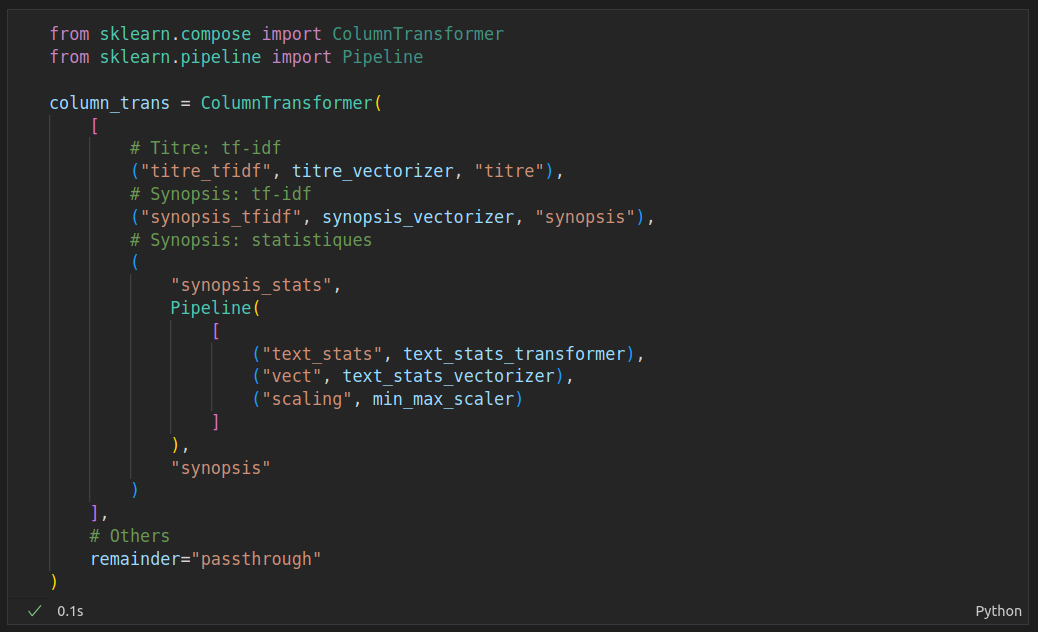
\includegraphics[scale=.3]{img/pipeline_1.png}
    \caption{Pipeline de pré-traitement des données}
    \label{pipeline_1}
\end{figure}

\subsection{Apprentissage Simple}
Avant tout apprentissage supervisé, il faut définir un jeu d'apprentissage et un jeu de test avec par exemple la méthode \textsf{train\_test\_split} de Scikit-Learn en spécifiant la proportion du jeu de données sélectionnée pour les données de test (typiquement: \textsf{test\_size=0.2}) et précisant \textsf{shuffle=True} pour que les données ne soient pas sélectionnées séquentiellement (ce qui pourrait impacter le résultat si le jeu de données est trié par classes).

\noindent
\begin{minipage}[!hc]{0.12\textwidth}
   \textbf{Remarque}
\end{minipage}
\vrule\enskip\vrule\quad\begin{minipage}{\dimexpr 0.87\textwidth-0.8pt-1.5em}
Le jeu de données \textit{allocine\_genres\_test.csv} correspond au jeu de validation qui ne sera utilisé qu'après avoir définitivement choisi la méthode de prédiction.
\end{minipage}

Il est alors possible de créer une nouvelle pipeline pour automatiser le pré-traitement et l'apprentissage \ref{pipeline_2}.

\begin{figure}
    \center
    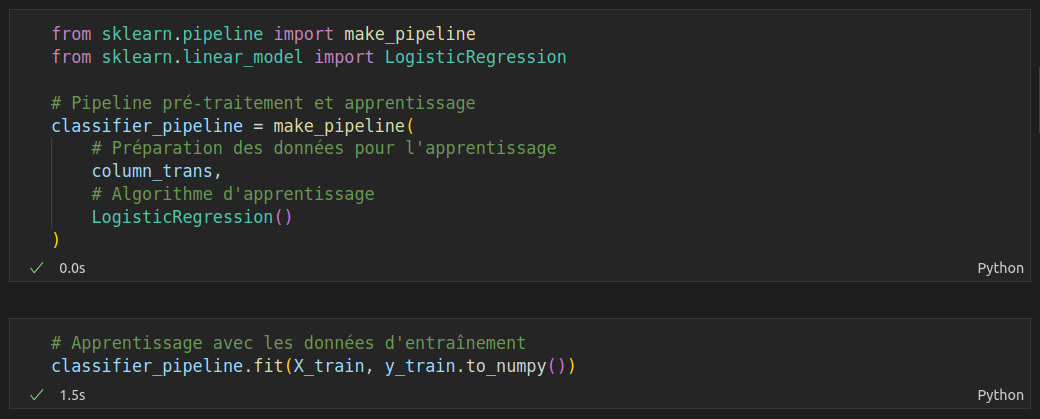
\includegraphics[scale=.3]{img/pipeline_2.png}
    \caption{Pipeline d'entraîenement d'un modèle de régression logistique}
    \label{pipeline_2}
\end{figure}

On peut ensuite faire des prédictions sur le jeu de test avec la méthode \textsf{predict} pour évaluer le modèle. Ce modèle de régression logistique donne une précision de 0.6 et un rappel de 0.61 (donc un score f1 de 0.6).

\subsection{Apprentissage par Plis et Comparaison des Algorithmes}
Comme vu précédemment, la taille et les individus sélectionnés pour entrainer le modèle peuevent avoir une influence sur la qualité de l'apprentissage. Pour contrer ce biais on peut utiliser des plis pour l'apprentissage: au lieu de diviser les données d'entraînement en un jeu d'entrainement et un jeu de test, on peut diviser les données d'entraînements en plusieurs plis qui seront tour à tour des données d'entraînement ou de test. Celà permet d'obtenir une idée de la performance moyenne du classifieur. On utilise la méthode _textsf{StratifiedKFold} de Scikit-Learn qui a la particularité de conserver la proportion d'individus de chaque classe dans les plis.

En utilisant cette méthode, on peut comparer le modèle de régression logistique avec d'autres algorithmes. Les meilleurs résultats proviennent d'un modèle de forêt aléatoire (précision proche de 0.7). \ref{omparaison}

\begin{figure}
    \center
    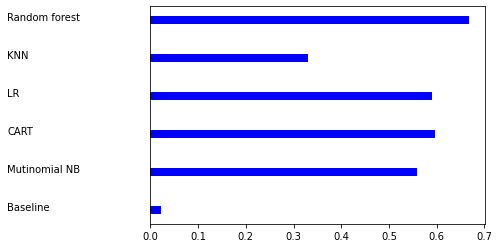
\includegraphics[scale=.5]{img/comparaison.png}
    \caption{Précision de différents algorithmes lors d'un apprentissage par validation croisée avec 5 plis}
    \label{comparaison}
\end{figure}